
\section{Motivation}
\label{sec:motivation}
 The ISPD gate-sizing contests aimed at producing robust solutions that could be easily integrated with an industrial flow. However, as pointed out in \cite{reis:16}, \cite{kahng:16} and \cite{kahng:14}, there still exists some significant challenges. As shown in \cite{kahng:14}, while the proposed solutions worked well in the framework of the contest, optimality was not guaranteed when technology nodes were changed. In this section we present an overview of the common bottlenecks that affect the robustness of the current solutions thus highlighting the need for the proposed \textit{MLTimer} solution. Our observations are as follows: 
\begin{itemize}
    \item \textbf{Initial configuration (line 2 of Algorithm~\ref{alg:naive})}: The algorithm needs to initially choose for every gate in their circuit, a cell of similar functionality from the multiple available cells specified in the standard cell library (typically three $V_t$ and ten $size$ options). Some of the recently proposed optimization techniques such as \cite{ozdal:12}, \cite{hu:12},\cite{li:12},\cite{flach:13}, and \cite{livramento:13} initialize all the gates in the netlist with a low power configuration using the largest $V_t$ and smallest $size$. However in an industrial flow this might not be possible as power optimization might be performed several times during each stage of the design flow. Initializing to a power optimal configuration  might create additional problems during the placement and routing stages as the final solution, while meeting the power constraints, might cause violations in the placement and routing constraints.    
  
    \item \textbf{Cost Function $\alpha(C)$}: Heuristic based solutions rely on cost functions to identify the candidate gate for optimization as seen in line 7 of Algorithm~\ref{alg:naive}.  However as seen in \cite{hu:12}, a single cost function for all designs might not be the best option. A poorly chosen cost function can lead to a sub-optimal solution and can increase the overall runtime of the algorithm. %elaborate talk about the impact of the cost function and 
    \item \textbf{Number of Static Timing Analysis (STA) calls (line $8$ of Algorithm~\ref{alg:naive})}: It can be seen from line $8$ of algorithm~\ref{alg:naive} that each replacement  necessitates an STA call to check whether the replacement has caused any timing violations. The number of STA calls made during the iterative process largely contributes to the overall runtime overheads. 

\end{itemize}

\noindent Thus, it is important to note that the quality of any leakage optimization heuristic is affected by the initial configuration, cost function and number of STA calls. We present a few empirical observations and inferences that can be leveraged to improve the above three factors.

\noindent {\bf Observation I}

\noindent Initializing each gate in the netlist  with random choices of both $size$ and $V_t$ (heterogeneous configuration) yielded better solutions in terms of  leakage power, delay and run time than the traditional approach. This is because, as we move to lower nanometer technologies, the delay and power do not scale linearly with $size$ and $V_{t}$. As a result, using a sub-optimal initial configuration might necessitate additional optimizations such as delay recovery, fixing slew and capacitance violations thereby resulting in a large running time. However the problem of finding the right initial configuration and the right cost function is impractical as it requires solving the entire TC-DSP in the initial stage. However as shown in Table~\ref{Tab:tab1}  several circuits can be seen to share \textit{structurally similar} sub-circuit patterns. Two sub-circuits are said to be \textit{structurally similar} if there exists an isomorphism (one-to-one mapping of vertices and edges) between them.  We leverage this observation to find the best possible initial configuration for one instance of the sub-circuit and  reuse the same for other occurrences of the sub-circuit. This has resulted in an initial configuration that causes significant reduction in both the overall execution time and the leakage power.
%A gate that has high negative slack could be subjected to delay optimization ($V_t$ downscaling or upsizing) whereas a gate with high positive slack could be subjected to power optimization. Hence, we need to identify the right operating conditions that affect the final configuration of the gate.

%if possible insert table to support the first point.

%\indent Consider the following example ~\ref{fig:example1}. Gate $G_1$ has same fanin and fanout gates but gets assigned different $V_t$ and $gate-size$ configurations. This is because the $G_1$ in ~\ref{fig:example1} has different slack than $G_1$ in ~\ref{fig:example2}. \textbf{It is not enough if the circuits share the same subcircuit pattern, they should also be under identical design conditions.}. This is illustrated in ~\ref{fig:example3} and ~\ref{fig:example4} where the same gate gets assigned same $V_t$ and $gate size$ even though they dont share a completely identical subcircuit pattern but because they share identical operating conditions.

%\indent From the examples and ~\ref{Tab:tab1} we see that different designs have several similarities which could be leveraged to predict a good initial configuration. While we might not be able to predict the exact final solution, the predicted solution can be used as a starting point for optimization. 



\begin{table*}[!t]
\centering
    \caption{Table showing the number of shared patterns across benchmarks. Each pattern is formed by using the gate along with its fanins and fanouts. The values highlighted in bold represent the total number of possible patterns for that particular benchmark. Element i,j represents the number of overlapping patterns of benchmark i in benchmark j.}
    \label{Tab:tab1}

    \begin{tabular}{ |p{2.2cm}| p{1cm}| p{1.2cm}| p{1.7cm} |p{1.4cm} | p{1.2cm}|p{1.4cm}|p{1.4cm}|p{1.4cm}|}
\hline
        \textbf{ Benchmark} & \texttt{DMA} & \texttt{pci} &\texttt{des\_perf} &\texttt{vga\_lcd} &\texttt{b19} &\texttt{leon3mp} &\texttt{netcard} & \texttt{ShaktiC} \\ \hline
    \texttt{DMA}       & \textbf{23,109} & 19,663          & 20,558           & 15,439           & 21,899           & 17,703           & 18,225           & 20,330           \\ \hline
\texttt{pci}       & 14,898          & \textbf{29,844} & 29,015           & 28,845           & 29,284           & 26,426           & 26,463           & 22,316           \\ \hline
\texttt{des\_perf} & 90,475          & 86,729          & \textbf{102,427} & 83,768           & 96,677           & 56,599           & 56,535           & 72,306           \\ \hline
\texttt{vga\_lcd}  & 15,439          & 25,316          & 27,339           & \textbf{147,812} & 41,068           & 69,696           & 58,099           & 100,034          \\ \hline
\texttt{b19}       & 182,984         & 166,217         & 181,228          & 166,372          & \textbf{212,674} & 141,619          & 139,733          & 156,877          \\ \hline
\texttt{leon3mp}   & 470,252         & 460,774         & 484,694          & 436,798          & 467,000          & \textbf{540,352} & 538,939          & 495,941          \\ \hline
\texttt{netcard}   & 813,634         & 809,793         & 834,303          & 785,423          & 796,790          & 860,397          & \textbf{860,949} & 777,582          \\ \hline
\texttt{ShaktiC}   & 120,422         & 86,762          & 72,306           & 100,034          & 134,521          & 94,361           & 115,425          & \textbf{174,756} \\ \hline
 \end{tabular}
    
\centering

\end{table*}



\begin{table*}[!t]
\centering
    \caption{Table showing the relative number of shared patterns across benchmarks. Each pattern is formed by using the gate along with its fanins and fanouts. The values highlighted in bold represent the total number of possible patterns for that particular benchmark.  Element i,j represents the percentage of overlapping patterns of benchmark i in benchmark j.}
    \label{Tab:tab13}

    \begin{tabular}{ |p{2.2cm}| p{1cm}| p{1.2cm}| p{1.7cm} |p{1.4cm} | p{1.2cm}|p{1.4cm}|p{1.4cm}|p{1.4cm}|}
\hline
        \textbf{ Benchmark} & \texttt{DMA} & \texttt{pci} &\texttt{des\_perf} &\texttt{vga\_lcd} &\texttt{b19} &\texttt{leon3mp} &\texttt{netcard} & \texttt{ShaktiC} \\ \hline
   \texttt{DMA}       & 100 & 85  & 89  & 67  & 95  & 77  & 79  & 88  \\ \hline
\texttt{pci}       & 50  & 100 & 97  & 97  & 98  & 89  & 89  & 75  \\ \hline
\texttt{des\_perf} & 88  & 85  & 100 & 82  & 94  & 55  & 55  & 71  \\ \hline
\texttt{vga\_lcd}  & 10  & 17  & 19  & 100 & 28  & 47  & 39  & 68  \\ \hline
\texttt{b19}       & 86  & 78  & 85  & 78  & 100 & 67  & 66  & 74  \\ \hline
\texttt{leon3mp}   & 87  & 85  & 90  & 81  & 86  & 100 & 100 & 92  \\ \hline
\texttt{netcard}   & 95  & 94  & 97  & 91  & 93  & 100 & 100 & 90  \\ \hline
\texttt{ShaktiC}   & 69  & 50  & 41  & 57  & 77  & 54  & 66  & 100 \\ \hline 
 \end{tabular}
    
\centering

\end{table*}


% \begin{figure} [!h]
% \begin{circuitikz} \draw %[scale=0.5\textwidth]
% %\begin{minipage}{0.5\textwidth}
% (0,2) node[and port] (myand1) {\footnotesize$G_1$ ($SV_t$)}
% (0,0) node[and port] (myand2) {$G_2$($SV_t$)}
% (2,1) node[or port] (myor) {$G_3$($SV_t$)}
% (4,2) node[and port] (myand3){$G_4$($SV_t$)}
% (4,0) node [and port] (myand4){$G_5$($SV_t$)}
% (myand1.out) -- (myor.in 1)
% (myand2.out) -- (myor.in 2)
% (myor.out)--(myand3.in 1)
% (myor.out)--(myand4.in 1);

% \end{circuitikz}
% \qquad
% \begin{circuitikz} \draw %[scale=0.5\textwidth]
% (0,2) node[and port] (myand1) {$G_1$}
% (0,0) node[and port] (myand2) {$G_2$}
% (2,1) node[or port] (myor) {$G_3$}
% (4,2) node[and port] (myand3){$G_4$}
% (4,0) node [and port] (myand4){$G_5$}
% (myand1.out) -- (myor.in 1)
% (myand2.out) -- (myor.in 2)
% (myor.out)--(myand3.in 1)
% (myor.out)--(myand4.in 1);
% %\end{minipage}
% \end{circuitikz}
% \caption{Consider Gate $G_1$ in both the circuits. $G_1$ has the same fanin and fanout gates but gets assigned different $V_t$ and $gate size$}
% \label{fig:example1}

% \end{figure}






% \begin{circuitikz} \draw
% (0,2) node[and port] (myand1) {}
% (0,0) node[and port] (myand2) {}
% (2,1) node[xnor port] (myxnor) {}
% (myand1.out) -- (myxnor.in 1)
% (myand2.out) -- (myxnor.in 2);
% \end{circuitikz}
% \caption{Consider Gate $G_1$ in both the circuits. $G_1$ has the same fanin and fanout gates but gets assigned different $V_t$ and $gate size$}
% \label{fig:example3}

% \begin{circuitikz} \draw
% (0,2) node[and port] (myand1) {}
% (0,0) node[and port] (myand2) {}
% (2,1) node[xnor port] (myxnor) {}
% (myand1.out) -- (myxnor.in 1)
% (myand2.out) -- (myxnor.in 2);
% \end{circuitikz}
% \caption{Consider Gate $G_1$ in both the circuits. $G_1$ has the same fanin and fanout gates but gets assigned different $V_t$ and $gate size$}
% \label{fig:example4}

\noindent {\bf Observation II:}

\noindent A traditional greedy heuristic for the TC-DSP involves the following two stage validation process for every replacement,
\begin{itemize}
\item {\it Local validation stage:} In this stage a gate ($g$) with the highest slack is assigned the next slower version ($V_t$ upscaled or $size$ reduced) to reduce the leakage power, without violating the timing constraint of $g$.
\item {\it Global validation stage:} The assignment of the entire circuit is validated by performing an incremental STA  and the arrival times/slacks are updated for all gates\footnote{Usually arrival times are associated with a net. 
In this paper, we represent the arrival time of a gate as the arrival time at the output of the gate}.
\end{itemize} 

\noindent It is interesting to note that in a slack-based greedy heuristic algorithm as described in~\cite{mok:12}, the gates that are higher in the ordering in the current iteration are successively replaced {\it with a high probability} in the next few iterations. We call this correlation between iterations as {\it iterative correlation}. Applying the greedy heuristic on the \texttt{c432} benchmark circuit from the ISCAS benchmark suite, where the gates were ordered in the decreasing order of slack at the end of each iteration, we see that the gates $51, 59, 70$ and $67$ that were in the top $5$ before iteration $1$, got replaced in successive iterations in the same order as given below. Here $\pi_i$ denotes the ordering of gates at the end of iteration $i$. The integers in the lists below denote the gate IDs. The gates that are {\it underlined} are the ones which get replaced in the respective iterations. It was also observed that the algorithms spend a majority of their running time in the global validation stage.\footnote{It can be noted that Gate $51$ is at the top of the list for both $\pi_1$ and $\pi_2$, as it had large amount of positive slack even after replacement in iteration $1$ and that the standard cell library used has more than two $V_t$ versions.} 
\vspace{0.1cm}
% * <sristisravan@gmail.com> 2017-06-28T07:47:57.575Z:
% 
% explain a bit on c432 and b14, maybe in footnote.. i didn't understand this terminology
% 
% ^.
\\
\noindent $\pi_1$: $\underline{51}$  $52$  $59$ $70$ $67$ $72$ $71$ $58$ $74$ $65$ $56$\ldots\\
$\pi_2$: $\underline{51}$ $52$ $59$ $70$ $67$ $72$ $71$ $58$ $74$ $65$ $56$\ldots\\
$\pi_3$: $\underline{59}$ $70$ $67$ $72$ $71$ $58$ $74$ $65$ $56$ $52$ \ldots\\
$\pi_4$: $\underline{70}$ $67$ $59$ $72$ $71$ $58$ $74$ $65$ $56$ $52$\ldots\\
$\pi_5$: $\underline{67}$ $59$ $72$ $71$ $58$ $70$ $74$ $65$ $56$ $52$\ldots

\vspace{0.1cm}

\noindent \noindent{\textbf{ Inference}}: One of the inferences from the above observation is that there exists a scope for reducing the run-time of the algorithm by exploiting the iterative correlation to postpone the global validation. In other words, the STA can be performed  after {\it multiple} gate replacements ({\it lazy timing evaluation}) in contrast to performing the same after every single gate replacement. This in turn,  significantly reduces the number of STA runs and thereby, the running time of the entire algorithm. To empirically justify the above inference, the following experiment was conducted. The greedy heuristics in~\cite{mok:12} was employed on the \texttt{c432} circuit with one gate being replaced in each iteration. We define $\pi^{'}_i = (gr_1, gr_2, gr_{i-1}, g_i, g_{i+1} ....)$, where 
$gr_j$, $1 \leq j < i$, denote the gate replaced in iteration $j$, and $g_k$, $k \geq i$ are the gates in decreasing slack values at iteration $i$.  
We then construct the matrix $\pi^{'} = \{\pi_1^{'}; \pi_2^{'}; \dots\}$. The {\it autocor} command in {\it GNU Octave} software is used to find the correlations between the rows in $\pi_i^{'}$. The autocorrelation function used in this experiment is shown in Equation~\ref{eqn:autocor}, 
where $i$ stands for the iteration number and $r$ for number of gates being replaced in each iteration.
\begin{equation} \label{eqn:autocor} \rho_{i}^{r} = corr(\pi_i,\pi_{i+r}) \end{equation}

\begin{figure}[!t]
\begin{center}
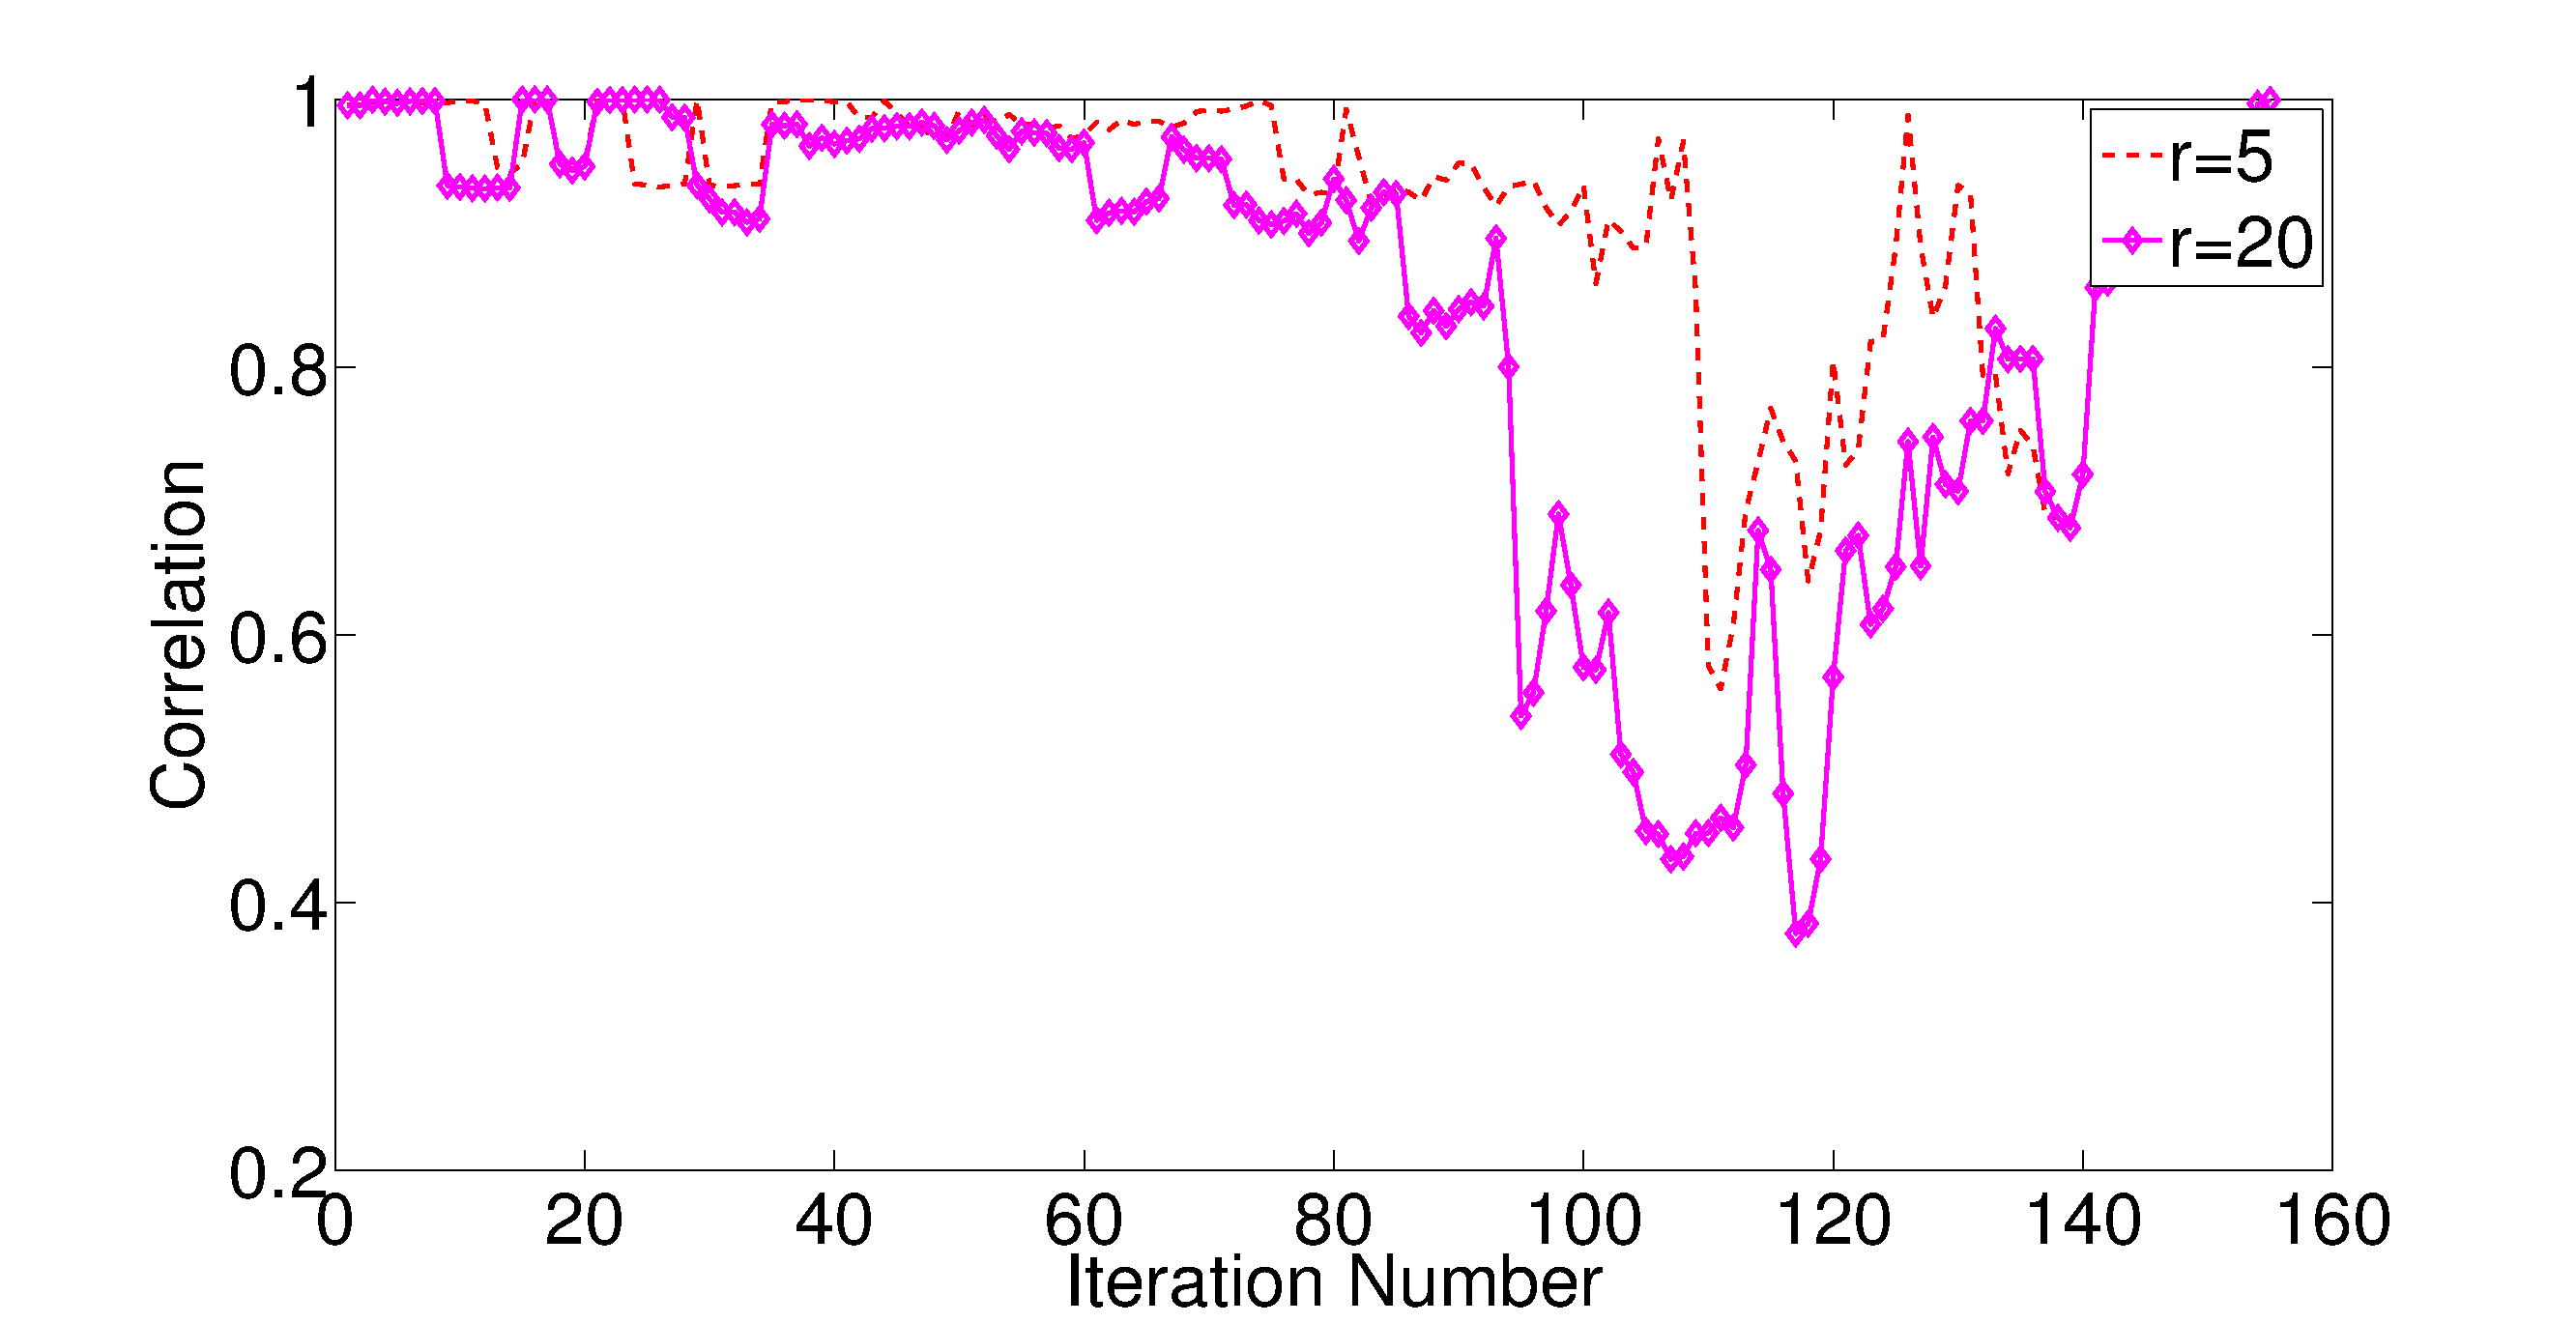
\includegraphics[scale=0.2]{Chapter3/fig/c432_correlation_between_ordering_replacements_with_throwngates.pdf}
\caption{X axis: $i$, Y axis: $\rho(i,i+r)$, where $i$: iteration number and $r$ : number of gate replacements per each iteration for 
\texttt{c432} circuit}
\label{fig:c432-corr}
\end{center}
\end{figure}
\noindent Figure~\ref{fig:c432-corr}
shows the autocorrelation plot of rows of $\pi^{'}$.
The Y-axis shows the correlation and X-axis the iteration number.
Each waveform on this plot shows how the correlation changes in successive iterations.

\noindent From figure~\ref{fig:c432-corr} we see that though there is scope for reducing the runtime by replacing several gates in each iteration, the optimal number of gates $r_{i}^{opt}$ to be replaced in each iteration varies and is not known beforehand. Hence there is a need to define metrics to compute the value of $r_{i}^{opt}$ effectively.\\
\noindent {\bf Observation III:} \\
It is important to note the impact of replacing multiple gates in a single iteration. In order to quantify the impact of replacing multiple gates in a single iteration we define two metrics:

\begin{itemize}
    \item {\it Backtrack (line number $10$ of Algorithm~\ref{alg:naive}) }: In case of a timing violation during a replacement the current replacement needs to be undone and the arrival/required arrival times of all wires in the circuit have to be updated to the old values which it had before the lazy timing update at the end of last iteration. This procedure is referred to as \textit{backtrack}. A large number of backtracks essentially degrades the running time of the TC-DSP optimization algorithm. 

    \item {\it Gate replacement window ($r$) }: In Algorithm~\ref{alg:naive}, only one gate is replaced  with a different $V_t$/$size$ per iteration as seen in line $7$ of the algorithm. This can be increased to $r$ gates. Figure~\ref{fig:saturation-of-running-time} shows the plot of running time versus varying $r$. 
It can be seen here that the running time decreases with an increase in $r$. 
After certain value of $r$ ($r_{opt}$), it saturates and does not improve further. 
        This is because, a very high value of $r$ causes too many backtrack operations thereby saturating the running time of the algorithm. This behavior was observed for other circuits also, although the value of $r_{opt}$ was different 
in each case. In general, the value of $r_{opt}$ increases with the size of the circuit as shown 
in Figure~\ref{fig:ropt}. 
\end{itemize}
\begin{figure}[t]
\begin{center}
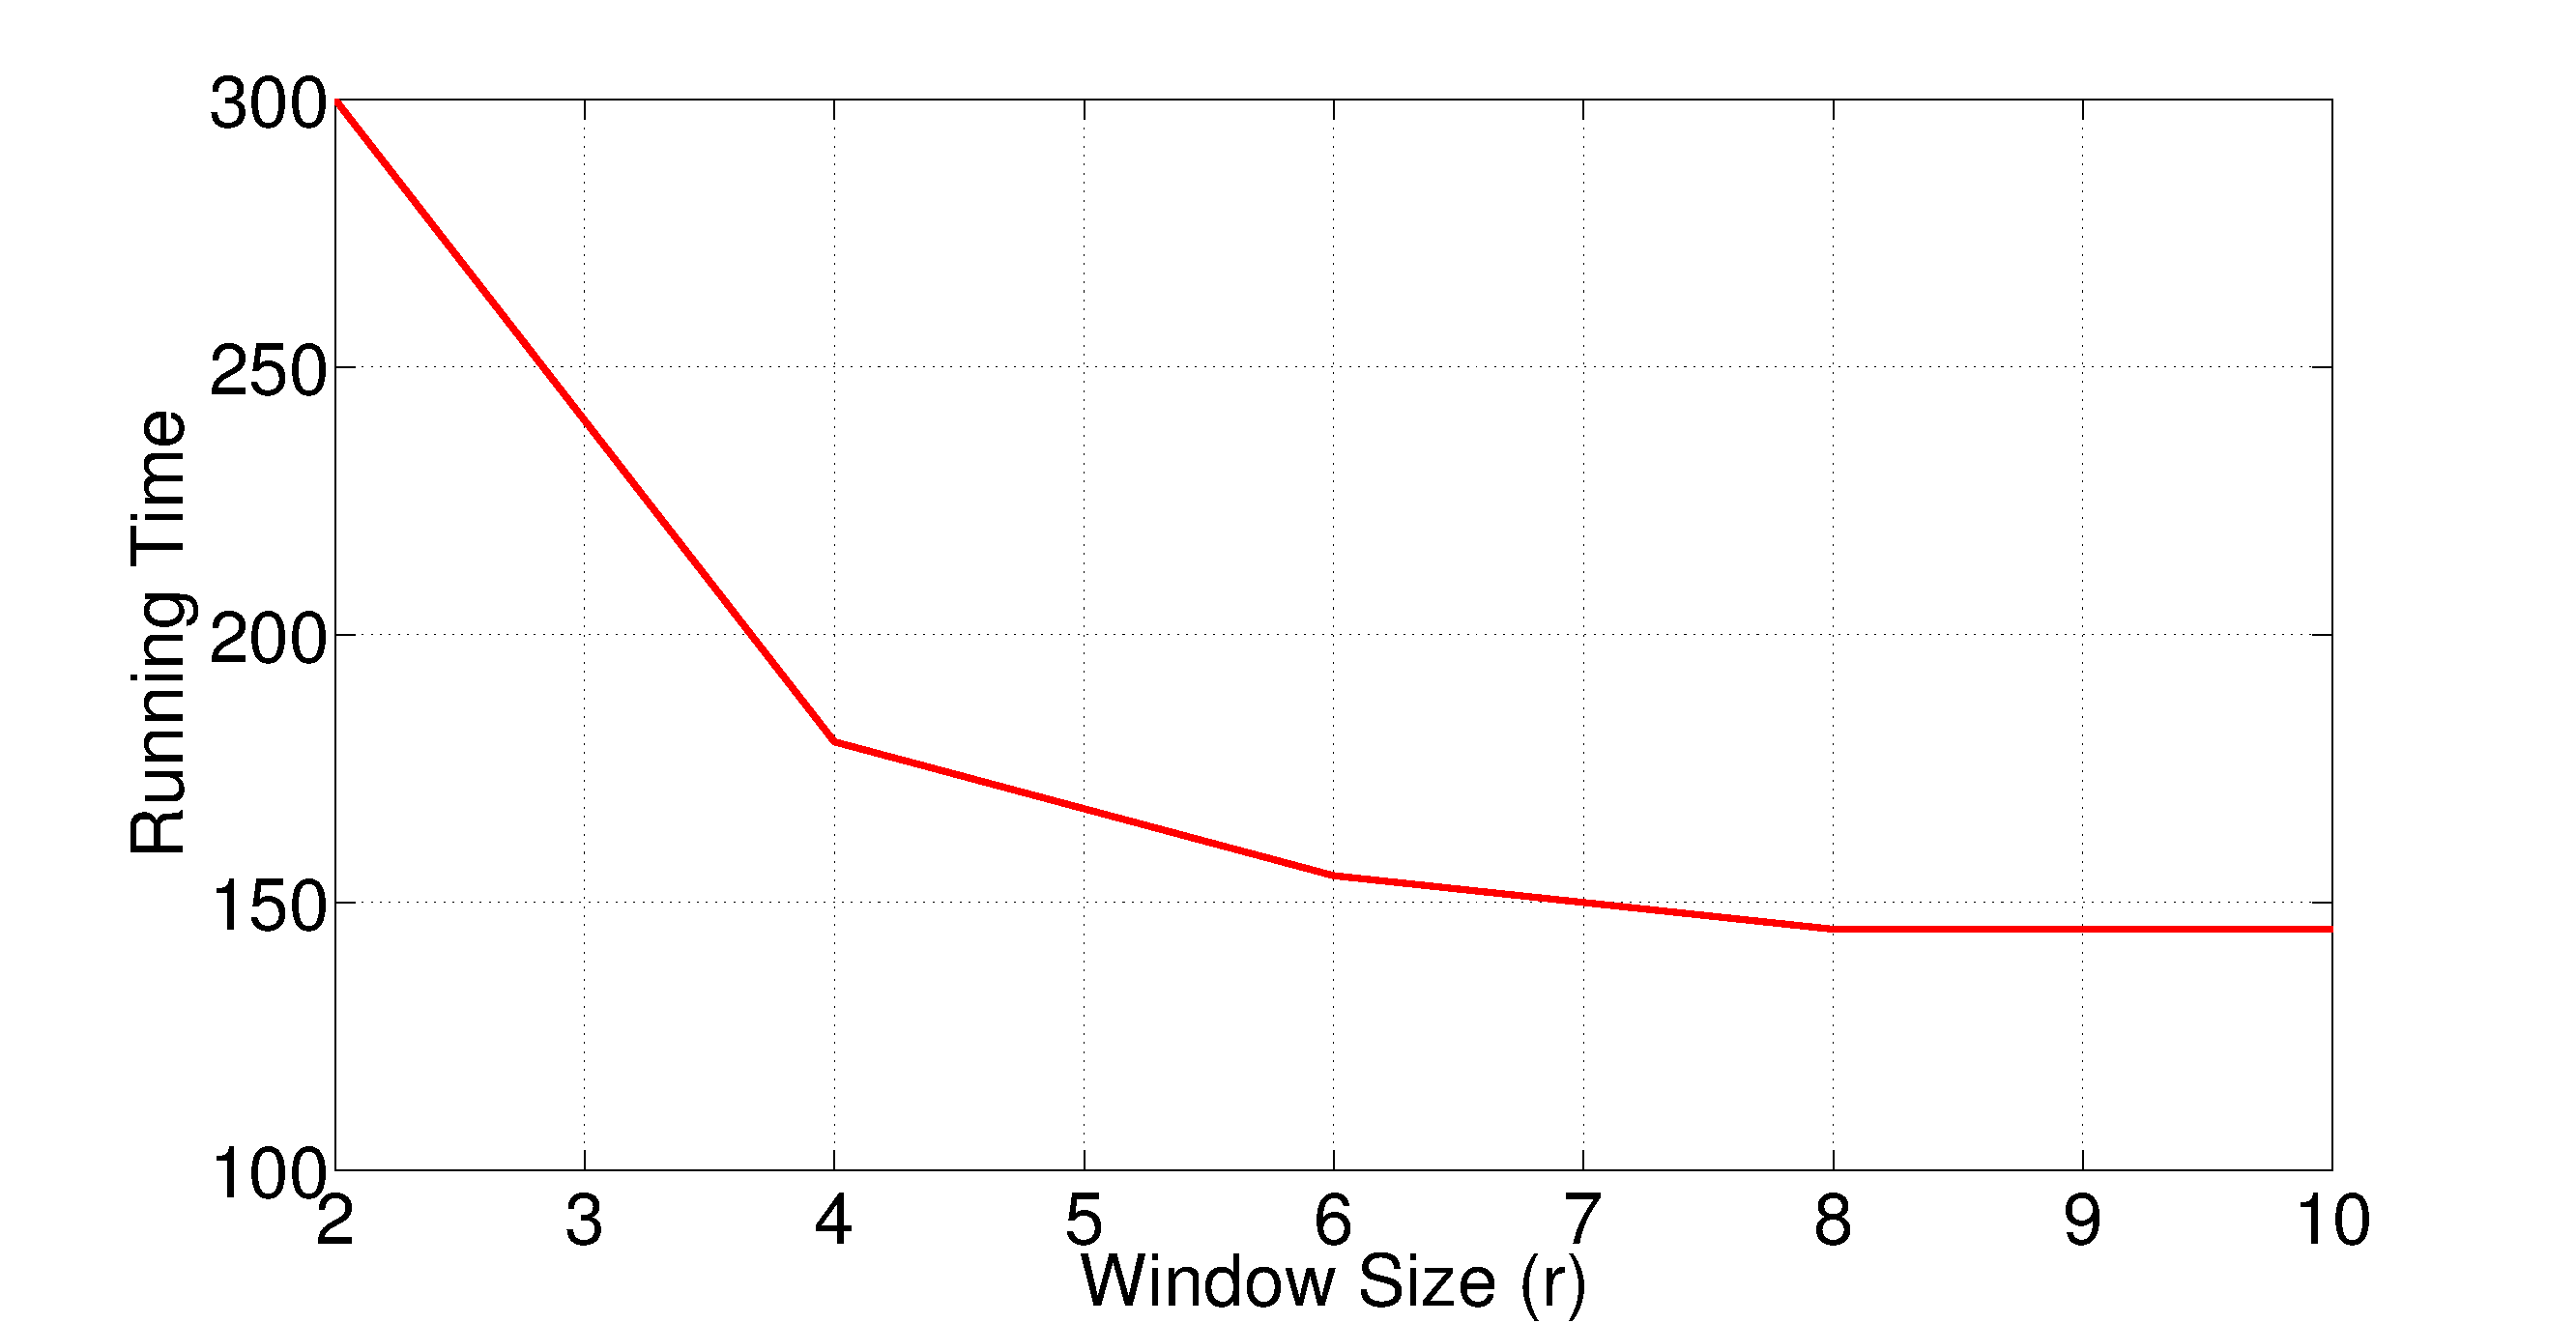
\includegraphics[scale=0.2]{Chapter3/fig/b14_running_time_vs_window_size.pdf}
\end{center}
\caption{Saturation of Running time (in s) with window size for \texttt{b14}}
\label{fig:saturation-of-running-time}
\end{figure}
\begin{figure}[t]
\begin{center}
\vspace{-0.2in}
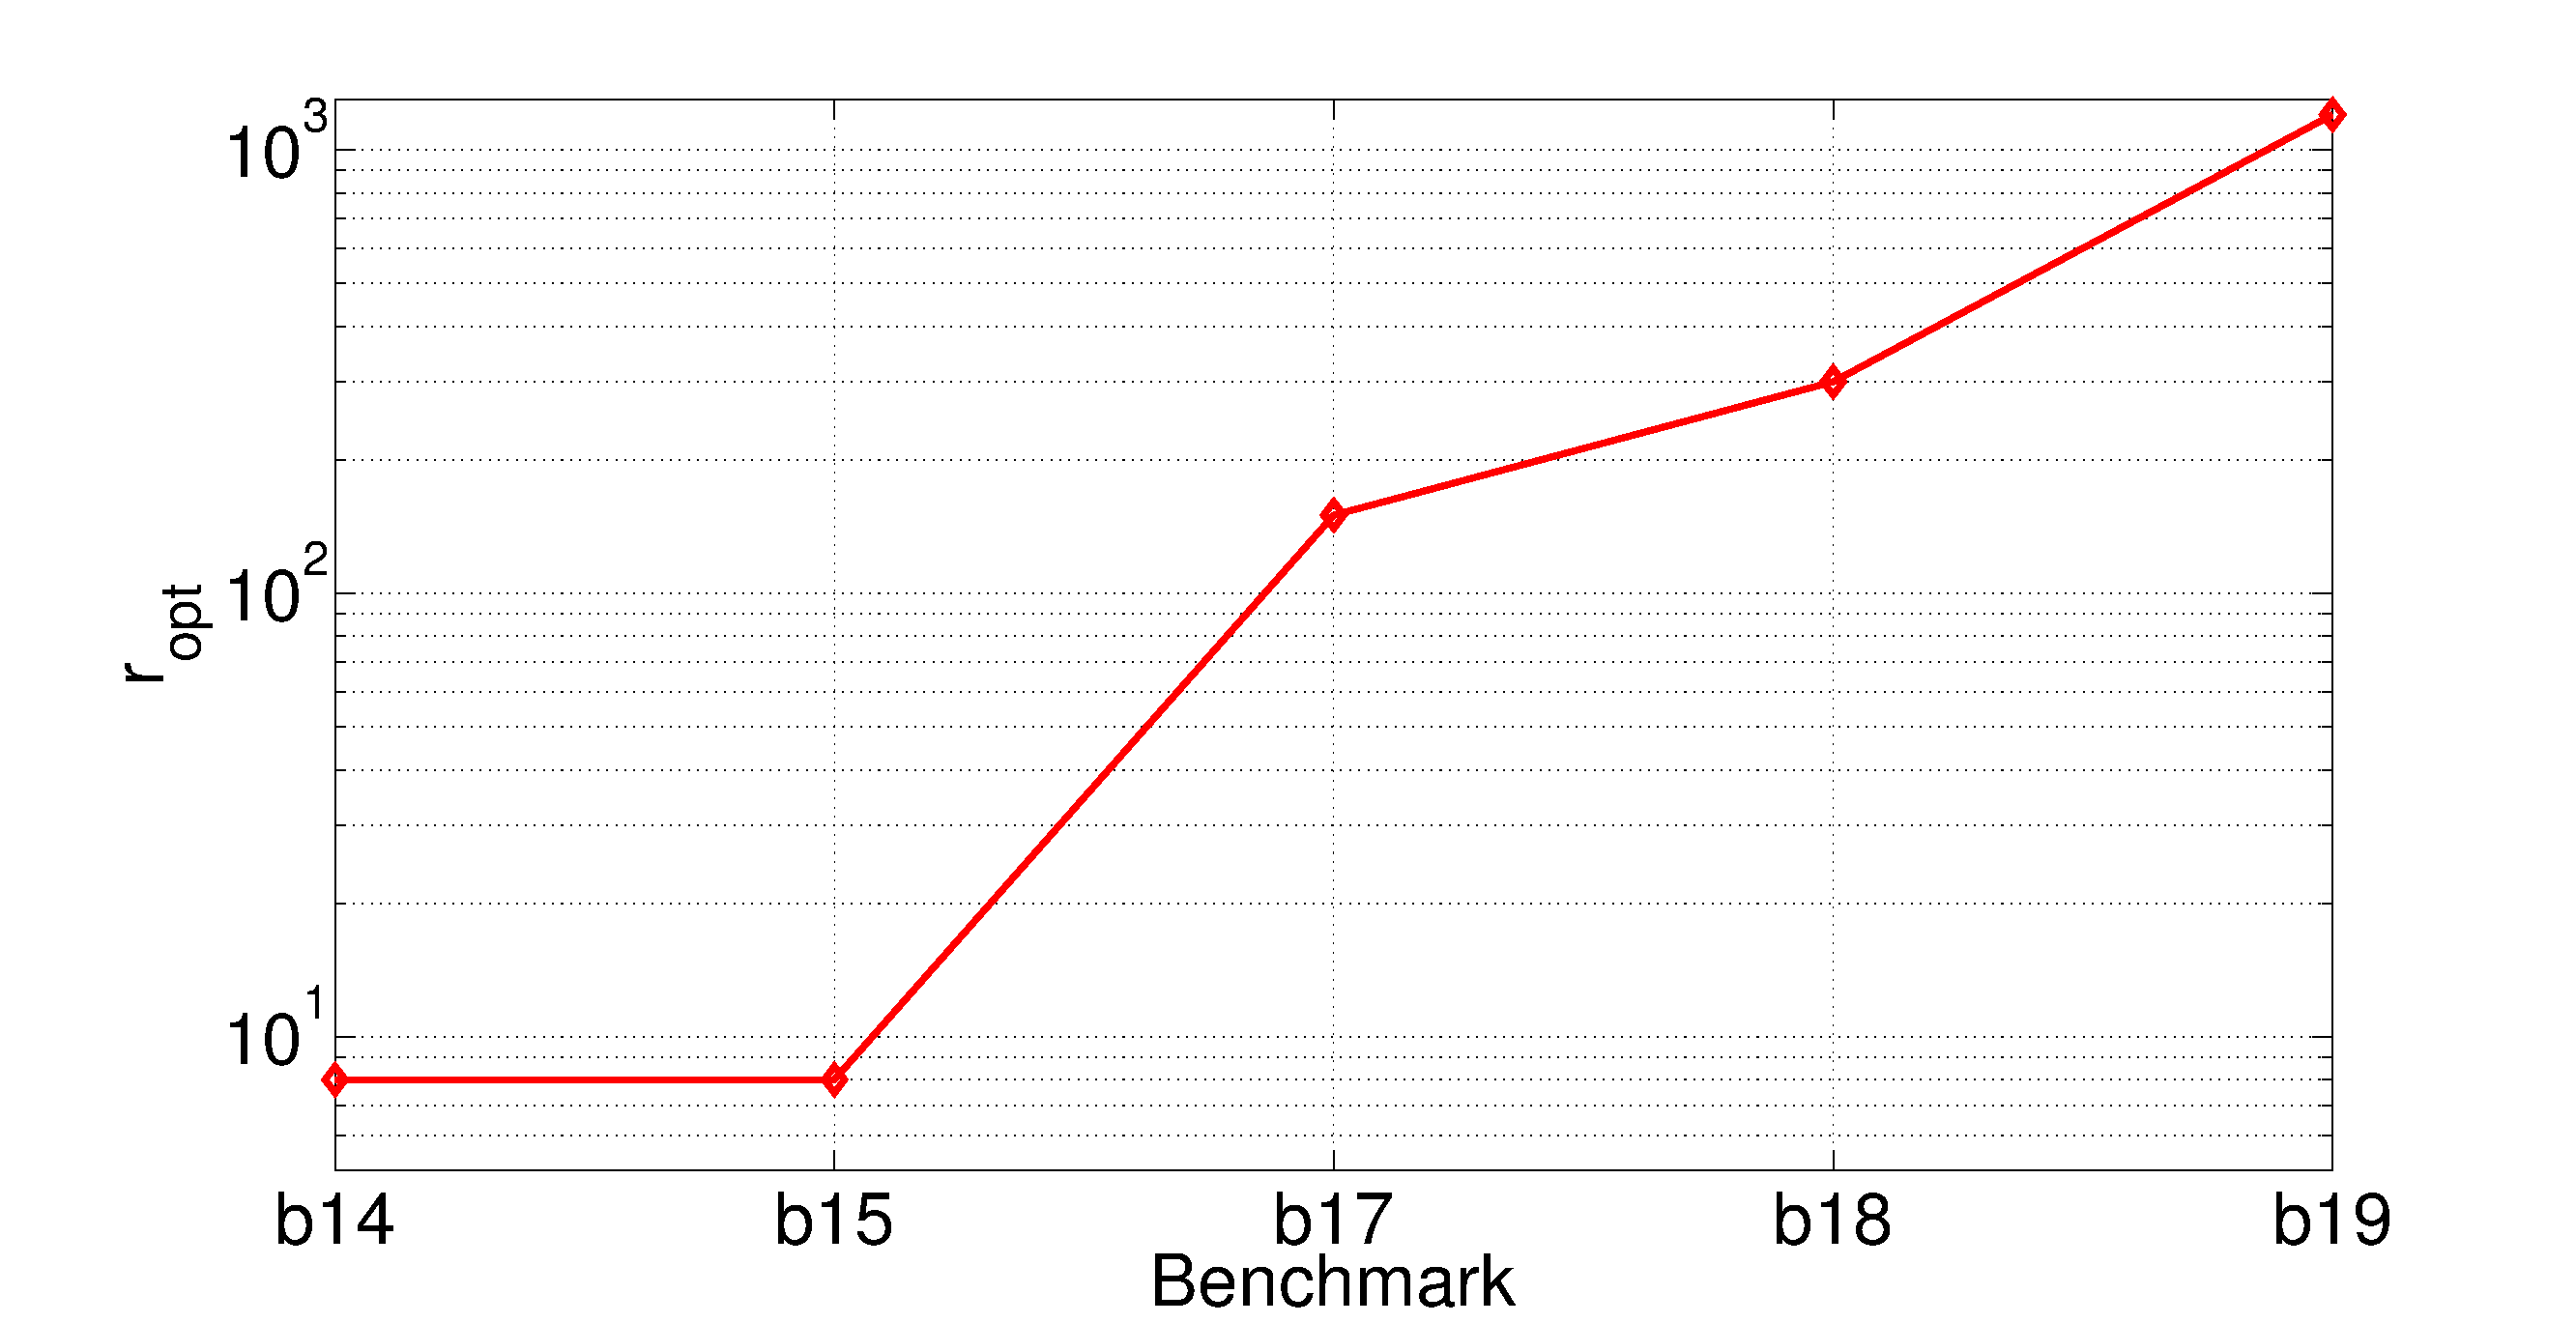
\includegraphics[scale=0.2]{Chapter3/fig/ropt.pdf}
\end{center}
\caption{$r_{opt}$ for different benchmarks}
\label{fig:ropt}
  %}
\caption{Figure showing the impact of varying $r$ over different benchmarks.}
\end{figure}


\noindent Figure~\ref{fig:c432-corr} shows that even for $r=20$, the correlation is very good, providing the opportunity for performing {\it lazy timing updates} between gate replacement iterations. If correlation is good for a certain value of $r$, it indicates that we can replace $r$ gates at a time, without violating timing. However, it impacts the run-time significantly if the iterative correlation is less. Further, it can also be observed in Figure~\ref{fig:c432-corr} that the correlation is not uniform across all iterations. Gates higher up in the ordering considered in the first few iterations have a high degree of correlation, whereas gates considered in the middle exhibit lower correlation. Hence replacing a fixed number of gates for each iteration may not effectively 
exploit the iterative correlation, leading to sub-optimal results. 


\noindent It can also be observed that while performing {\em lazy timing analysis}, an incremental-STA based update needs multiple {\em incremental STA runs}, one for each replacement. For a large $r$ , running one full blown STA (FSTA) run is much more efficient than running $r$ incremental-STA (ISTA) runs, 
to make the lazy timing update. For this reason, FSTA is employed for making the lazy timing updates during the  optimization.

\noindent \textbf{Inference}: The above observations can lead to the following inferences:

\begin{itemize}
\item Multiple gates can be replaced in a single iteration using {\it lazy timing analysis}.
\item It would be desirable to change the number of gates being replaced  in successive iterations, by exploiting the iterative correlation to 
effectively improve the algorithm running time, without compromising the solution quality.
\end{itemize}





\noindent From the above observations and inferences, we understand that a) multiple gates can be replaced 
in a single iteration using {\em lazy timing analysis} and that the optimal window size ($r$) for best 
savings in running time depends on the iteration. The next section explains how to adaptively vary $r$ to obtain the best savings in running time, without impacting solution quality. As seen in Table~\ref{Tab:tab1} we also see that two different circuits, irrespective of their sizes, can have many sub-circuits in common. This indicates that some of the solutions for smaller benchmarks can be reused for the larger benchmarks. However, the final $V_t$ and $size$ choice is dependent on several other factors apart from identical sub-circuits. Hence appropriate features need to be chosen so that the solutions for a benchmark can be leveraged while solving for others. To this end, we propose \textit{MLTimer} which uses the above observations to speed-up the leakage power optimization algorithm while improving the solution quality.
